
%(BEGIN_QUESTION)
% Copyright 2010, Tony R. Kuphaldt, released under the Creative Commons Attribution License (v 1.0)
% This means you may do almost anything with this work of mine, so long as you give me proper credit

This critical process vessel is equipped with {\it three} different level transmitters, all measuring the same liquid level, sending their respective signals to a {\it logic solver} control device that ``votes'' on the three signals to determine whether or not the process is operating safely.  The three level transmitters, however, each employ a different technology:

$$\includegraphics[width=15.5cm]{i04695x01.eps}$$

Transmitter LT-215a uses a hollow float on a metal rod to sense liquid level, and detects the float's position along the rod by means of timing sound waves sent through the metal rod.  Transmitter 215b senses differential pressure between the two nozzles (connection points to the vessel) as an indication of liquid level inside.  Transmitter 215c senses liquid level by a radio wave echoed off the liquid surface along a metal rod called a waveguide.

\vskip 10pt

Explain why it is important for the reliability of this redundant measurement system to use different technologies.  Why not just use three identical transmitters instead?

\vskip 20pt \vbox{\hrule \hbox{\strut \vrule{} {\bf Suggestions for Socratic discussion} \vrule} \hrule}

\begin{itemize}
\item{} What specific information would we need to determine a SIL level value (1 to 4) for the safety instrumented function protecting this process vessel from overfilling?
\item{} Does the reliability of the pressure relief valve (PRV-93) in this process affect the SIL rating of the overfilling protective function?  Explain why or why not.
\item{} Explain how you would go about comprehensively {\it testing} this safety system to check for proper function.  Could you specifically test {\it dependability} versus {\it security}?  Why or why not?
\item{} For those who have studied level measurement, explain how each of the three level transmitters work.
\end{itemize}

\underbar{file i04695}
%(END_QUESTION)





%(BEGIN_ANSWER)


%(END_ANSWER)





%(BEGIN_NOTES)

Each level-measurement technology uses a completely different operating principle.  Therefore, {\it common-cause failures} are virtually eliminated.

\vfil \eject

\noindent
{\bf Prep Quiz:}

A critical temperature-measurement process uses three redundant temperature transmitters to measure the same physical point, but each transmitter uses a different type of sensing element (RTD vs. thermocouple vs. infra-red).  Why are three {\it different} types of sensors used instead of one common type?

\begin{itemize}
\item{} Different sensor types reduce the risk of common-cause failures
\vskip 5pt 
\item{} Using three different types of sensors is less expensive 
\vskip 5pt 
\item{} The engineer couldn't decide between three different sensor options
\vskip 5pt 
\item{} Identical sensor types would cause interference with one another
\vskip 5pt 
\item{} Temperature measurement accuracy is enhanced by using different sensors
\vskip 5pt 
\item{} It is impossible to use three sensors of one type at the same location
\end{itemize}

%INDEX% Safety, redundancy: multiple transmitters

%(END_NOTES)

